\section{RGB Model} 

  \begin{definition}[RGB]
    The \textbf{RGB} model is an additive color model that uses red, green, and blue as the primary colors. 
  \end{definition}

  \begin{figure}[H]
    \centering 
    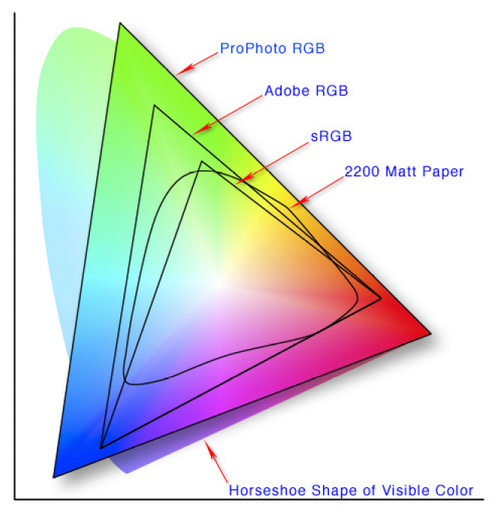
\includegraphics[scale=0.4]{img/colorspace.png}
    \caption{The gamut of visible colors w.r.t. the primary colors compared to gamuts of hardware in monitors. For visual convenience, all gamuts are projected into a 2-dimensional space.} 
    \label{fig:colorspace}
  \end{figure}

\subsection{Warmth}
